Analizując pomiary dla 4 laserów które przeprowadziłem, można wyciągnąć nastepujące wnioski:
\begin{itemize}
\item Sprawność różniczkowa laserów krawędziowych w funkcji zarówno prądu i mocy wejściowej jest większa, co
przedstawia wykres na rysunku ~\ref{fig:plot_eff}
\item Prąd progowy dla laserów krawędziowych jest większy od prądu progowego dla laserów VCSEL, co przedstawia wykres
na rysunku~\ref{fig:plot_temp_i_th}.
\item Także, sprawność całkowita w wyższych temperaturach jest większa, co możemy zobaczyć na wykresie przedstawionym na
rysunku~\ref{fig:plot_wall_eff}.
\end{itemize}
\section{Porównanie laserów}
\begin{figure}
\center
  \includegraphics[scale=0.30]{plot_common/plot_eff.eps}
  \caption{Wykres sprawności różniczkowej w funkcji prądu oraz mocy wejściowej.}
  \label{fig:plot_eff}
\end{figure}
\begin{figure}
\center
  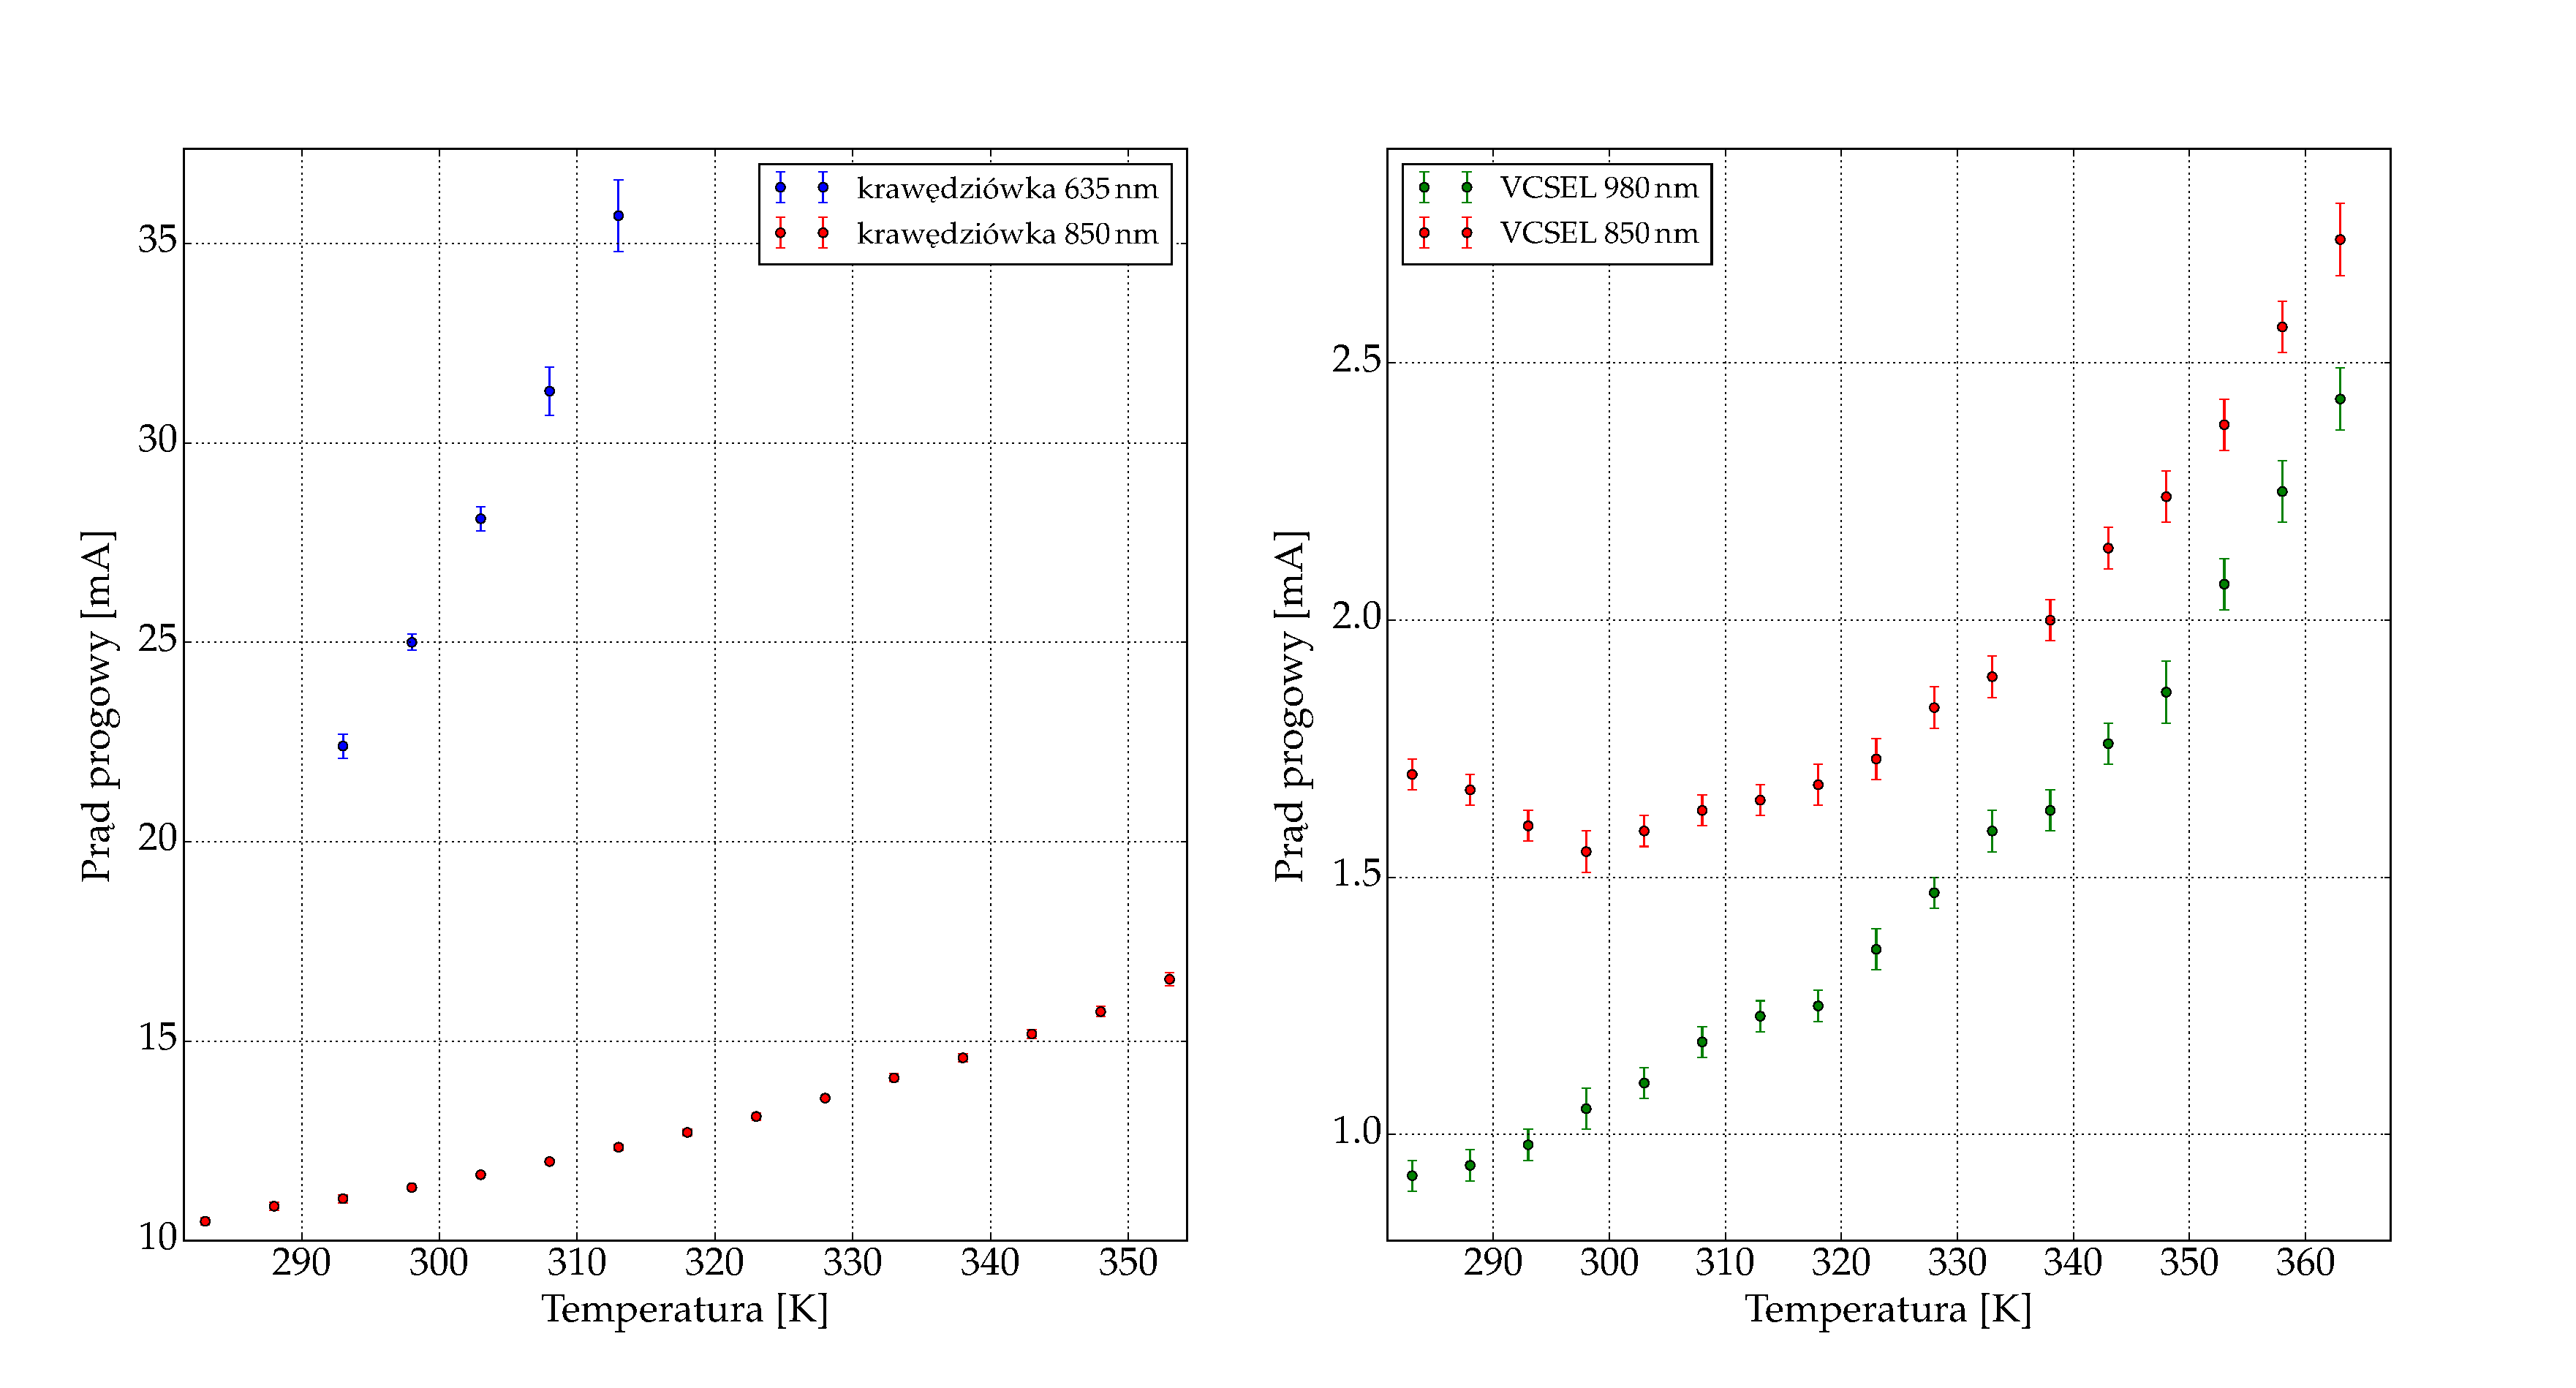
\includegraphics[scale=0.30]{plot_common/plot_temp_i_th.eps}
  \caption{Wykres prądu progowego od temperatury.}
  \label{fig:plot_temp_i_th}
\end{figure}
\begin{figure}
\center
  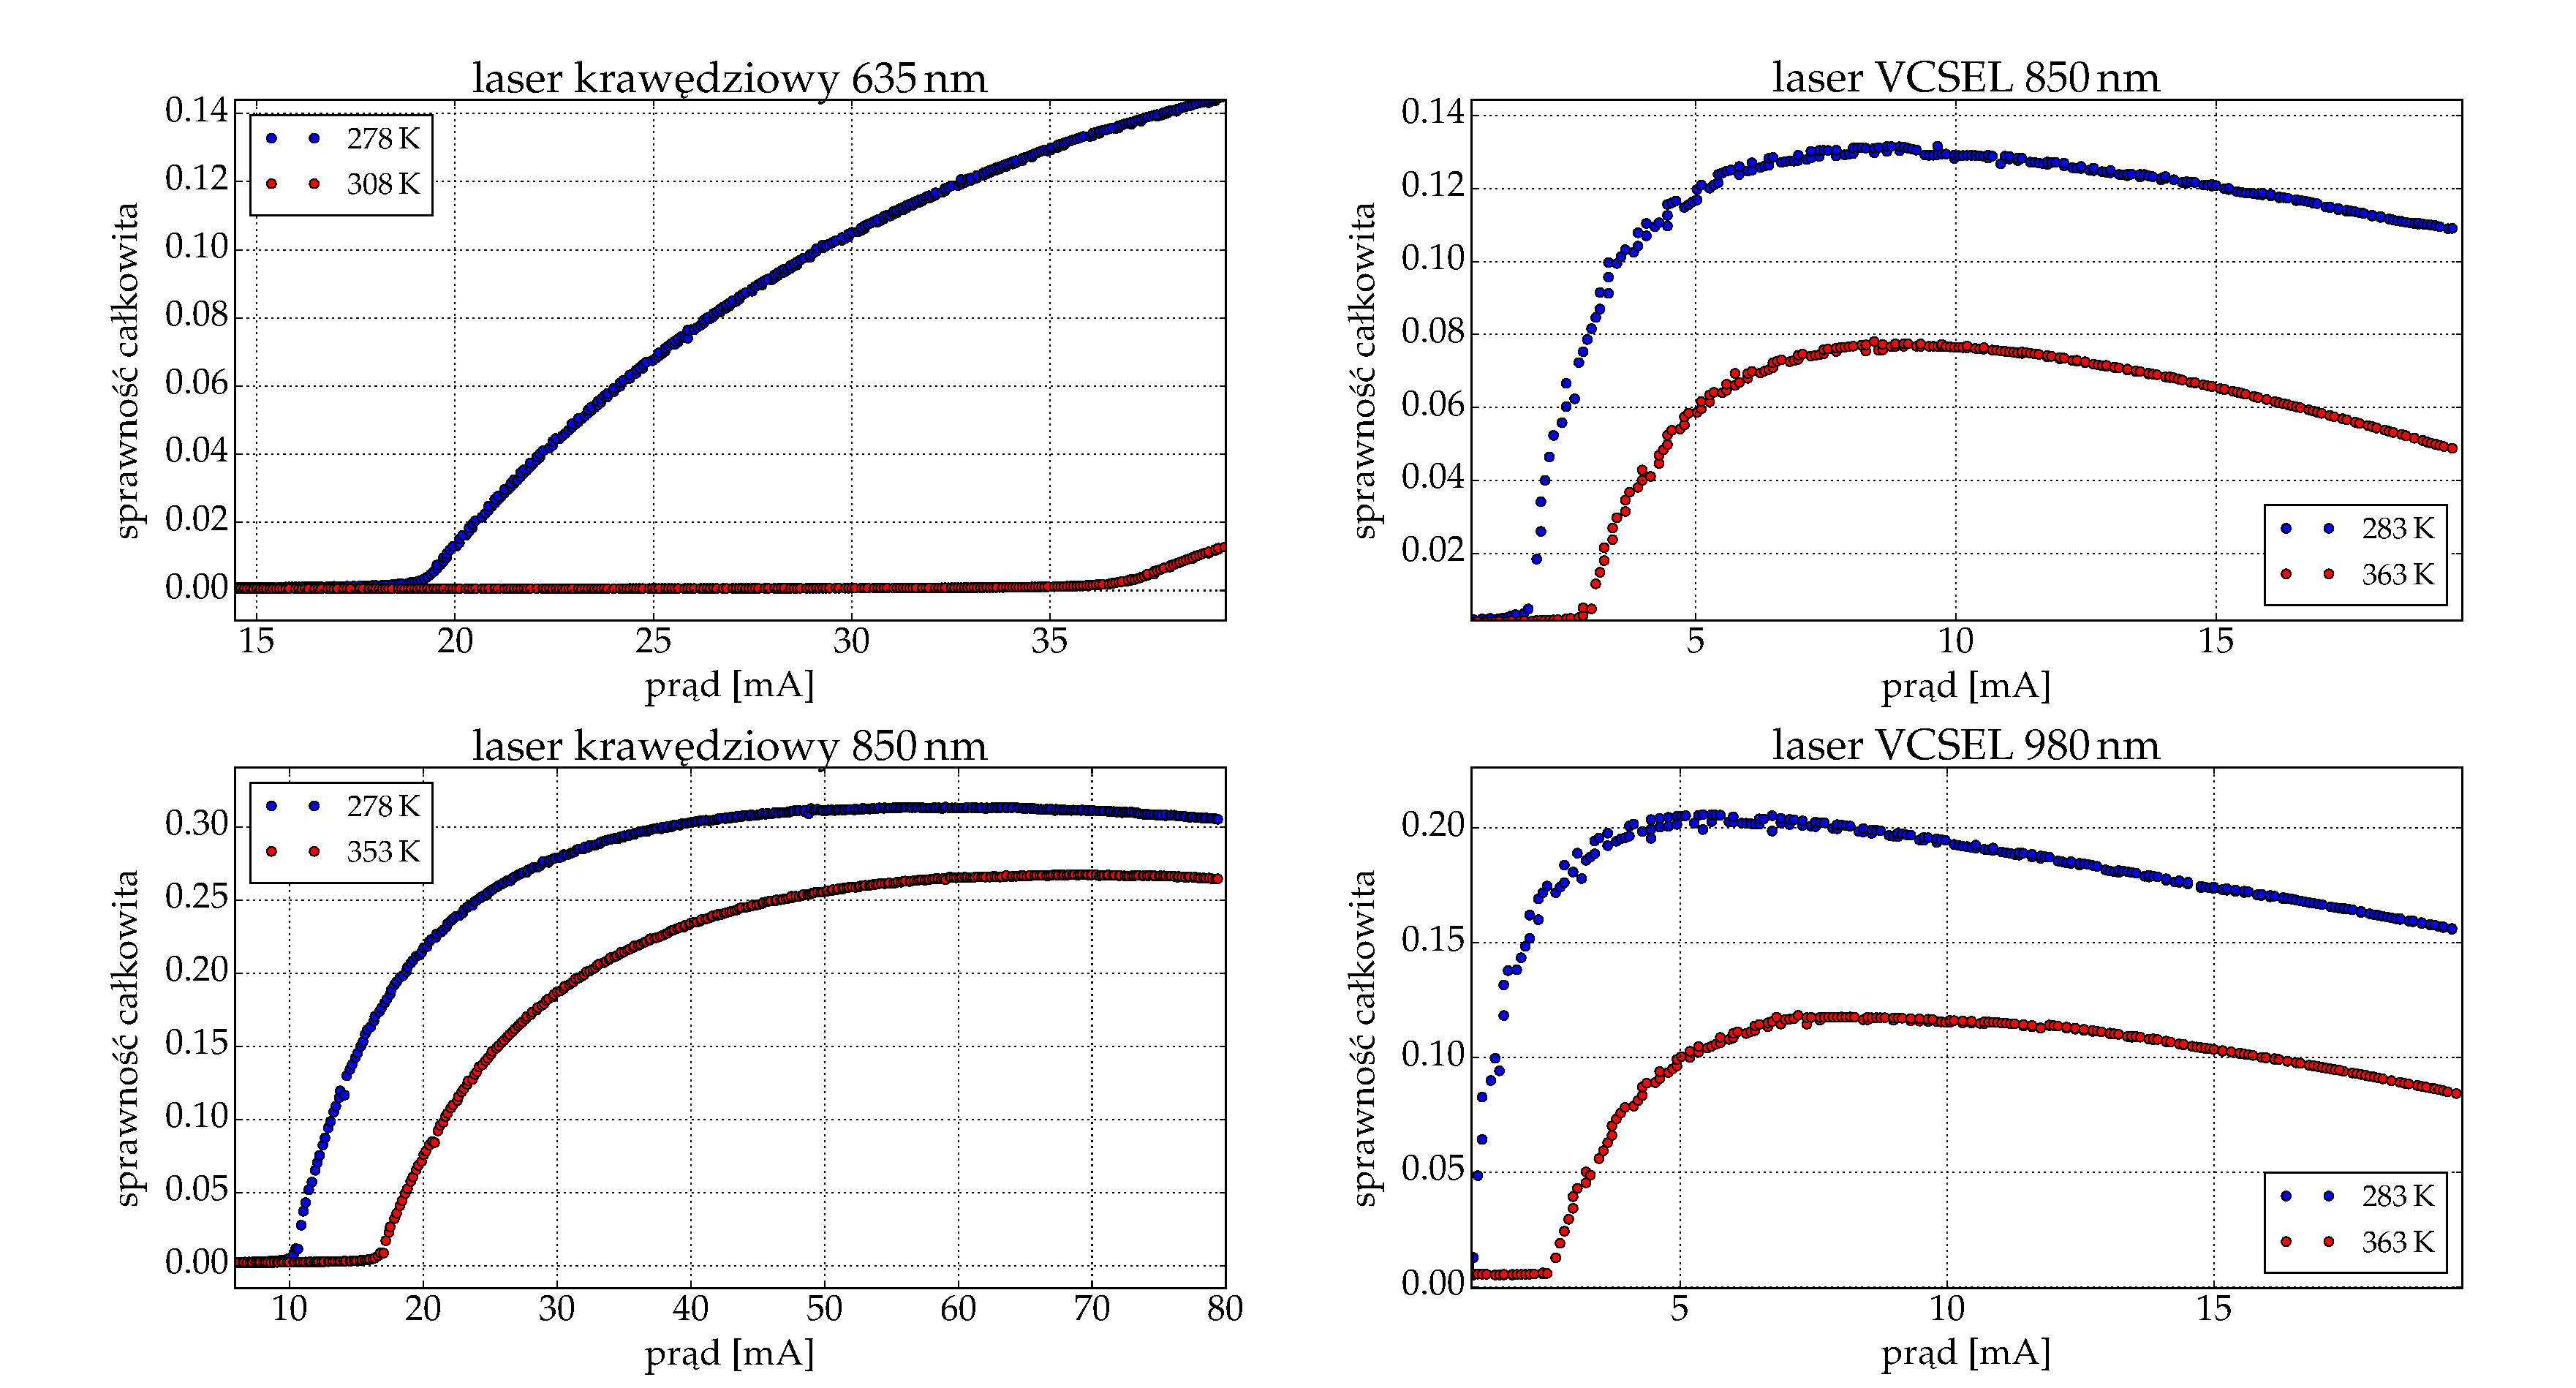
\includegraphics[scale=0.30]{plot_common/plot_wall_eff.eps}
  \caption{Wykres sprawności całkowitej w funkcji prądu.}
  \label{fig:plot_wall_eff}
\end{figure}
